\documentclass{article}
\usepackage{fontenc}
\usepackage[ngerman]{babel}
\usepackage[utf8]{inputenc}
\usepackage{graphicx}

\usepackage{datetime}
\newdateformat{myformat}{\THEDAY{ten }\monthname[\THEMONTH], \THEYEAR}

\begin{document}
	\begin{titlepage}
		\centering
		{\scshape\LARGE
			Ereignisdiskrete Systeme
			\par}
		\vspace{1.5cm}
		{\huge\bfseries Praktikum Blatt 1\par}
		\vspace{1.5cm}
		{\LARGE\itshape Jan Kristel, Alexandra Moritz\par}
		\vfill
			Aufsicht von Frau Rembold\par
			
		\vfill	
			{\large \today \par}	
		
	\end{titlepage}
	
	\tableofcontents
	\newpage
	\section{Aufgabe 1: MATLAB Grundlagen}
		\subsection{Was ist MATLAB?}
		Matlab ist eine Hochleistungssprache für technisches Rechnen. Es integriert Berechnung, Visualisierung und Programmierung in einer benutzerfreundlichen Umgebung, in der Probleme und Lösungen in vertrauter mathematischer Notation ausgedrückt werden. \\
		Typisch verwendet sind:
		\begin{itemize}
\item Mathematik und Rechnen
\item Entwicklung von Algorithmen
\item Modellierungssimulation und Visualisierung
\item wissenschaftliche und technische Grafiken
		\end{itemize}
Dies ermöglicht es Ihnen, viele, technische Rechenprobleme, insbesondere solche mit Matrix- und Vektorformulierungen, in einem Bruchteil der Zeit zu lösen, die benötigt würde, um ein Programm in einer skalaren nicht-interaktiven Sprache wie C oder Fortan zu schreiben. Der Name Matlab steht für Matrixlabor.
		\subsection{Wesentliche Komponenten der MATLAB-Oberfläche}
			\begin{figure}[h]
				\includegraphics[scale=0.45]{MATLAB_Übersicht_1_b.png}
				\caption{MATLAB Oberfläche}
				\label{fig2: MATLABOberflaeche}
			\end{figure}
	\newpage
			\begin{figure}
				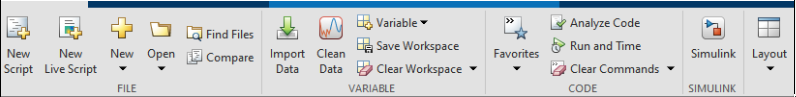
\includegraphics[scale=0.5]{TOOLStirp.png}
				\caption{Tool-Strip im Reiter "Home". Hier lassen sich neue Skripte erstellen oder vorhandene öffnen.}
				\label{fig3: ToolStrip_Home}
			\end{figure}		
			\begin{figure}
				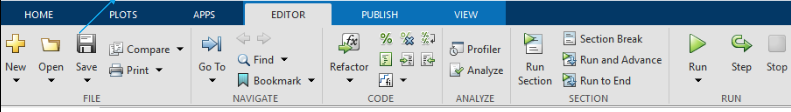
\includegraphics[scale=0.5]{TOOLStrip_Editor.png}
				\caption{Tool-Strip im Reiter "Editor". Mit "Run" lassen sich die Programme/Skripte starten, die man im Editor erstellt hat.}
				\label{fig3: ToolStrip_Home}
			\end{figure}	
			
		\subsection{\textit{Current Folder Browser} - Wozu? Was ist zu beachten?}
			Der Current Folder Browser zeigt Ordner und Dateien im aktuellen Arbeitsverzeichnis an. Man braucht es um den Zugriff auf die Dateien und Skripte zu erleichtern und um sicherzustellen das MATLAB die Dateien findet. Es ist wichtig die Dateien in der richtigen Stelle zu speichern, da die MATLAB-Programme standardgemäß im aktuellen Arbeitsverzeichnis ausgeführt werden. 
		
		\subsection{\textit{Comand Window} - Was verbirgt sich dahinter?}
			Das Command Window ist eine Konsole, die für die Eingabe von dem Benutzer verwendet wird und hier werden die MATLAB-Befehle eingegeben. Es wird auch eine Historie der davor eingegebenen Befehle gespeichert, sodass man sie immer wieder benutzen kann. 
			
		\subsection{\textit{Tool-Strip} - Was verbirgt sich dahinter?}
			Der Tool-Strip ist eine Symbolleiste, hier findet man auf häufig verwendete Funktionen. Es bietet beispielsweise schnellen Zugriff auf das Command Window oder die Hilfe-Funktionen. 
		
		\subsection{Zweck des \textit{Workspaces}}
			Der Workspace zeigt die aktuellen Variablen und ihre Werte an. Man kann es vergleichen mit einer Variablenansicht in anderen Programmieumgebungen. 
		
		\subsection{Möglichkeiten Information von \textit{MATLAB-Hilfe} zu bekommen}
			\begin{itemize}
				\item Die Online-Hilfe von MATLAB, die über der Webseite erreichbar ist 
				\item in MATLAB direkt die Hilfefunktion, die über der Schaltfläche „Hilfe“ auf der Symbolleiste aufgerufen werden kann. Oder durch Eingabe in der Kommandozeile mit „help“. 
			\end{itemize}
		
		\subsection{Simulink}
			\begin{itemize}
				\item MATLAB öffnen
				\item in der Commandozeile "simulink" eingeben
				\item oder über die Symbolleiste (Tool-Strip) Simlink starten
			\end{itemize}
		
		\subsection{\textit{Control System Tollbox} - Was ist das? Wo findet man sie?}
			
		
		\subsection{Stateflow}
			\begin{itemize}
				\item MATLAB öffnen
				\item in der Kommandozeile "stateflow" eingeben und "Enter" drücken.
			\end{itemize}
		
		
	\newpage	
	\section{Aufgabe 2: Bodediagramme}
		\begin{figure}[h]
 		 	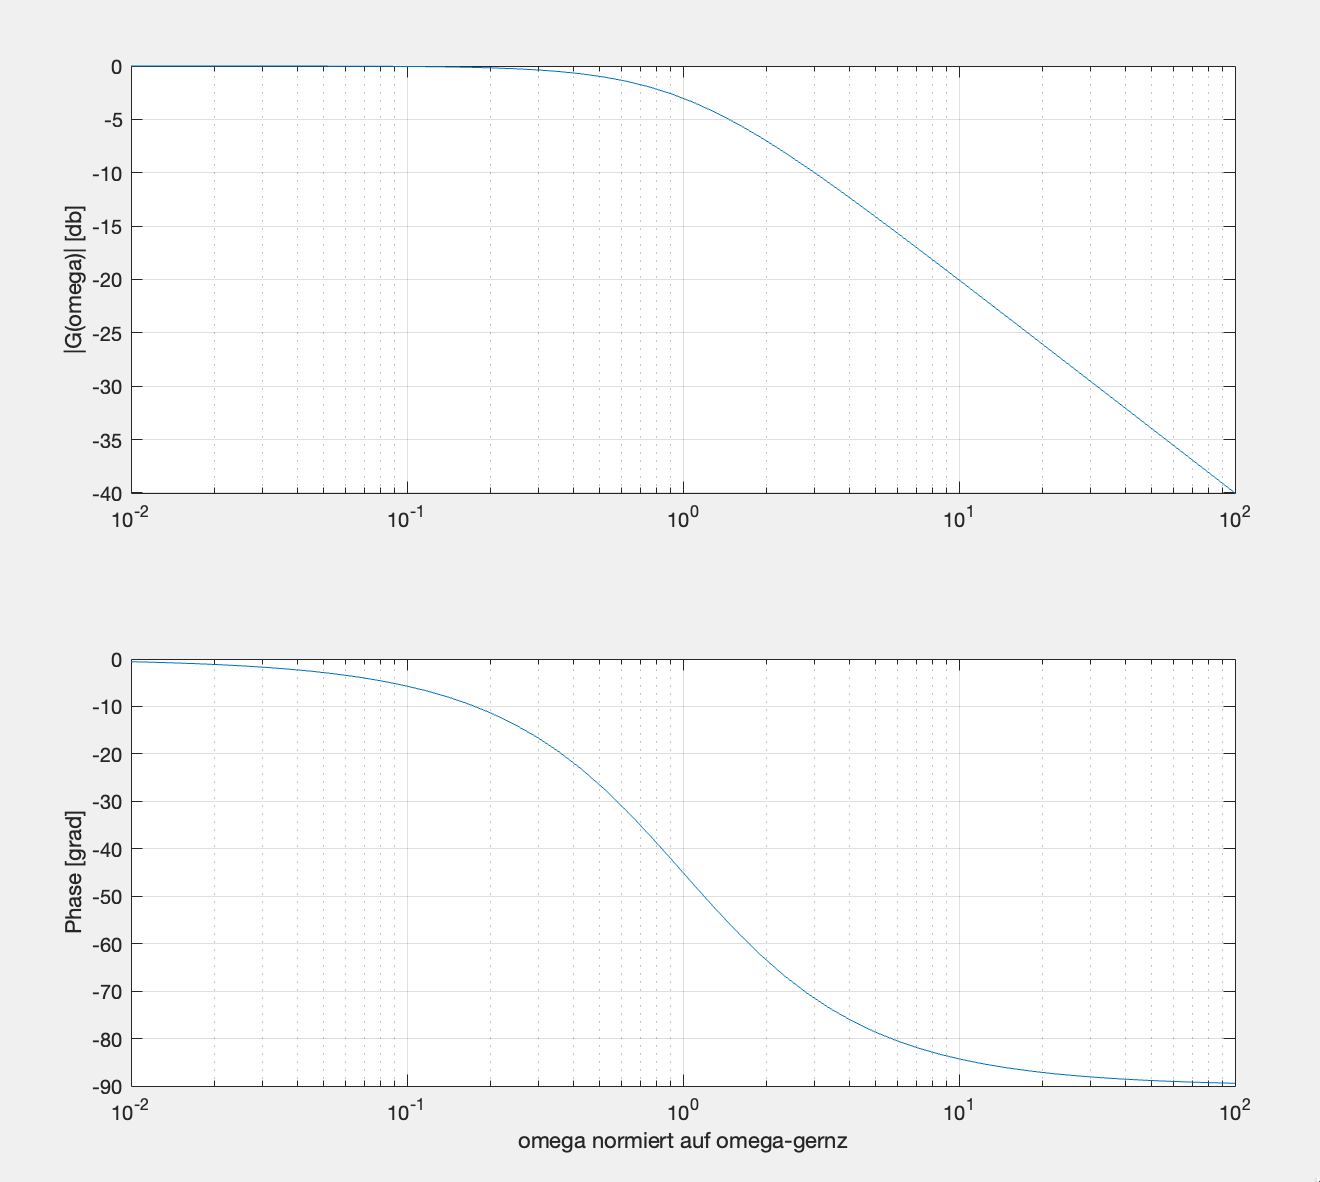
\includegraphics[scale=0.3]{Bodediagramme.png}
			\caption{Bodediagramme entstanden aus bodePT1.m}
			\label{fig1: Bodediagramm1}
		\end{figure}
		
		
		\subsection{Normierter Frequenzgang PT1-Glied}
		
		\subsection{Normierter Frequenzgang PT2-Glied}
	
	\newpage	
	\section{Aufgabe 3: Ortskurve}
	
	\newpage
	\section{Aufgabe 4: MATLAB Control System Toolbox}
	
\end{document}